%%%%%%%%%%%%%%%%%%%%%%%%%%%%%%%%%%%%%%%%%%%%%%%%%%%%%%%%%%%%%%%%%%%%%%%%%%%%%% 
\section {Simulation of muon decays in flight }

DIF simulation uses a standard multi-stage Mu2e simulation approach with
the stages defined as follows:

\begin{itemize}
\item
  stage 1: mu+ beam is traced to the DS entrance.
  TS3 collimator is rotated by 180 degrees.
  Total statistics: 5e8 POT (1000 segments x 500,000 events per segment).
\item
  stage 2: resampling in the DS by a factor of about x1000 (1600/1.52).
  The Ti degrader thickness varied from 2 mm to 5 mm with a step of 1mm.
  $\mu^+$'s were forced to decay within the proper time of 150 ns \cite{MU2E_41916_KRZYSZTOF}.
  Initial implementation of the technique had a bug: it has been implemented
  for $\mu^-$'s only.
  A proper time constraint for $\mu^+$'s has been added as a part of this study.
  Constraining the proper decay time increases the DIF simulation efficiency
  by $\sim$ x15 (see below).  
\item
  stage 3: digitization
\item
  stage 4: reconstruction and ntuple production.
\end{itemize}

The simulated statistics of the DIF is equivalent to $7.9 \times 10^{12}$ POT.
%%%%%%%%%%%%%%%%%%%%%%%%%%%%%%%%%%%%%%%%%%%%%%%%%%%%%%%%%%%%%%%%%%%%%%%%%%%%%%
\subsection {Constraining the muon proper decay time - validation}

Figure~\ref{figure:dif_proper_time_constraints} shows distributions in the $\mu^+$
decay vertices for different choices of the simulation constant $T_{max}$ constraining
the muon decay times.
One can see that, as expected, reducing the value of the constant leads to the increased
yield of muon decays. 

Down to $T_{max}=100$ ns, the distributions have very similar shapes.
For $T_{max}=50$ ns, the Z distribution shows the effect of the constrained
decay time. Based on Figure~\ref{figure:dif_proper_time_constraints} and aiming
to be conservative, we choose the value of $T_{max}=150$ ns, although it is possible
that using $T_{max}=100$ ns might have provided an additional gain in efficiency of about x1.5
without introducing any significant side effects

\begin{figure}[H]
  \begin{tikzpicture}
    \node[anchor=south west,inner sep=0] at (0,0.) {
      % \node[shift={(0 cm,0.cm)},inner sep=0,rotate={90}] at (0,0) {}
      \makebox[\textwidth][c] {
        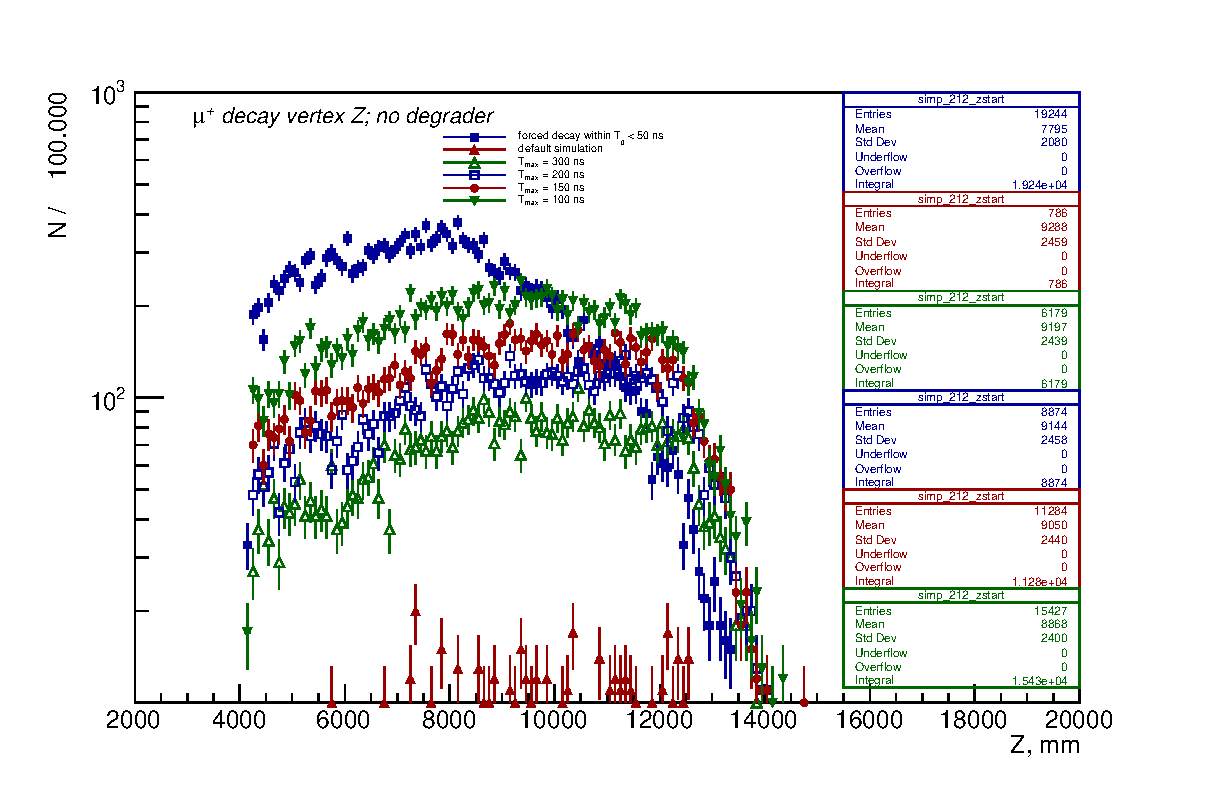
\includegraphics[width=0.9\textwidth]{pdf/figure_03501}
      }
    };
    % \node [text width=8cm, scale=1.0] at (14.5,0.5) {$\mu_B$, expected background mean};
    % \node [text width=8cm, scale=1.0, rotate={90}] at (1.5,7.5) { $S_{D}$, ``discovery'' signal strength  };
  \end{tikzpicture}
  \caption{
    \label{figure:dif_proper_time_constraints}
    Distribution of the $\mu^+$decay time in the DS
  }
\end{figure}

\begin{figure}[H]
  \begin{tikzpicture}
    \node[anchor=south west,inner sep=0] at (0,0.) {
      % \node[shift={(0 cm,0.cm)},inner sep=0,rotate={90}] at (0,0) {}
      \makebox[\textwidth][c] {
        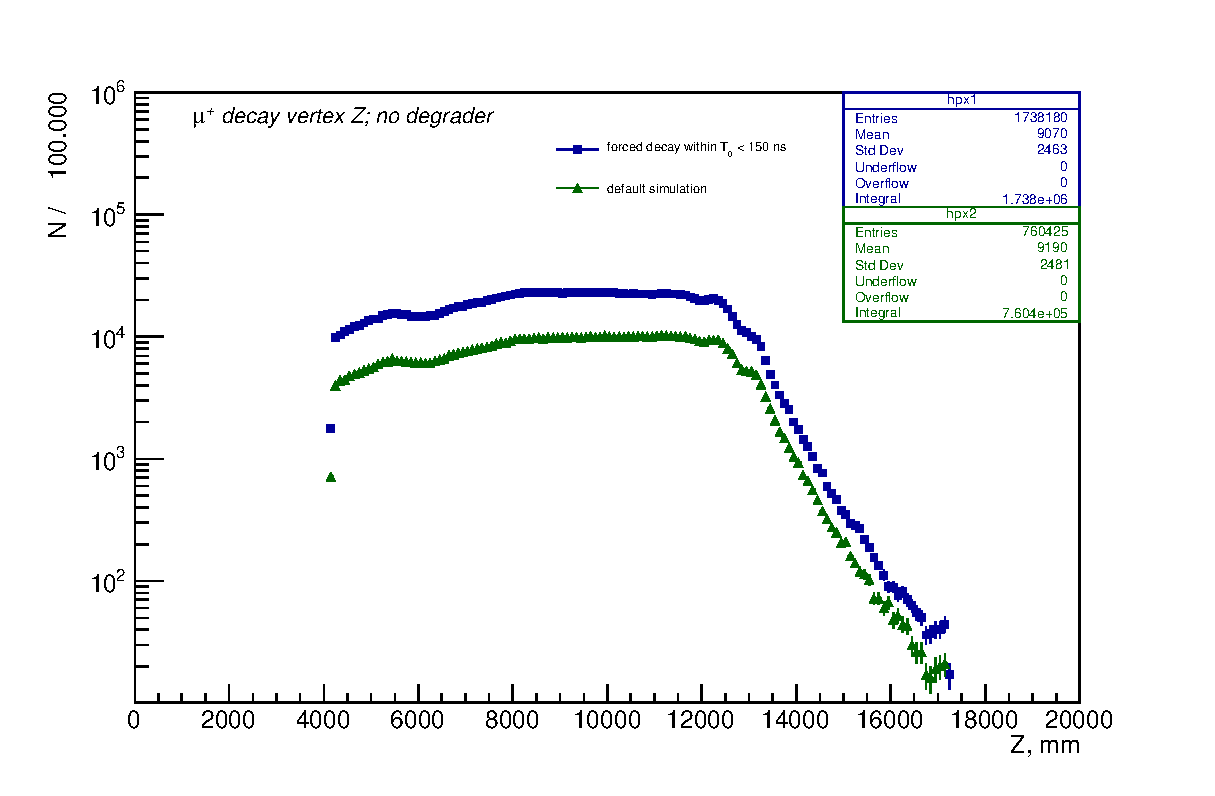
\includegraphics[width=0.55\textwidth]{pdf/figure_03401}
        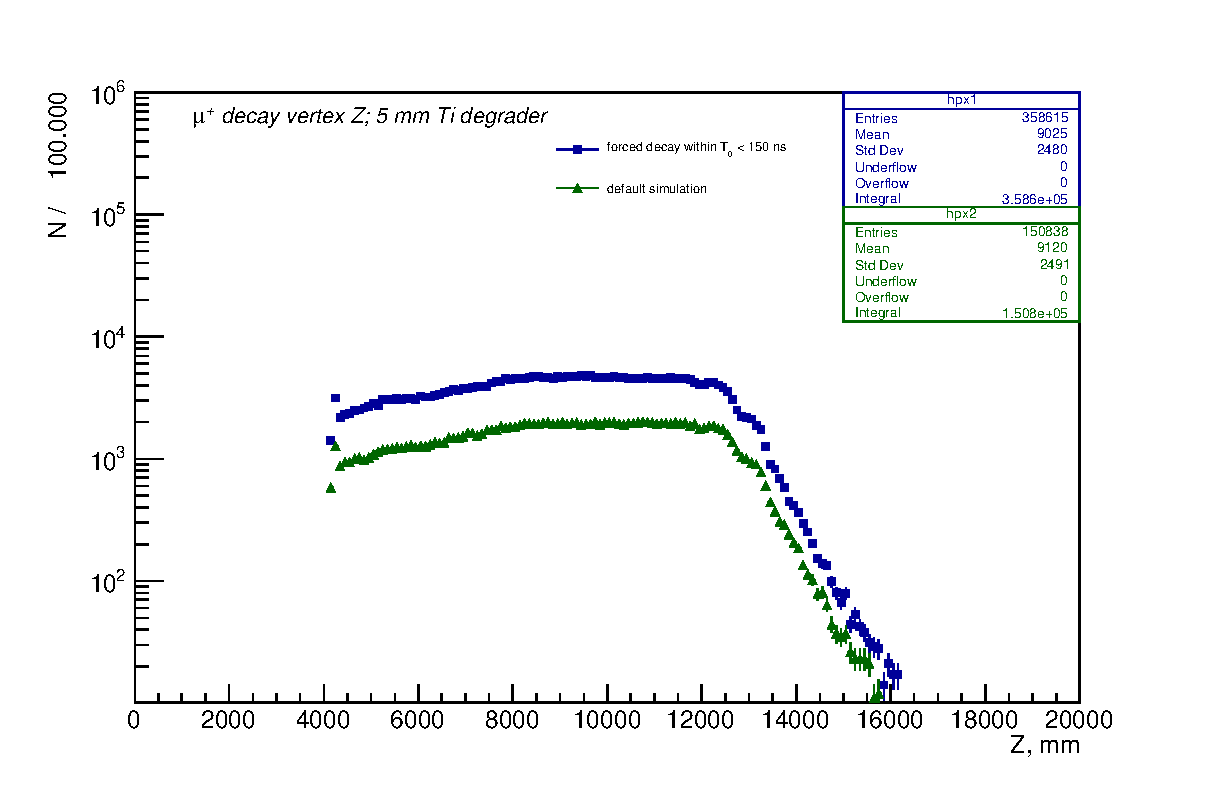
\includegraphics[width=0.55\textwidth]{pdf/figure_03451}
      }
    };
    % \node [text width=8cm, scale=1.0] at (14.5,0.5) {$\mu_B$, expected background mean};
    % \node [text width=8cm, scale=1.0, rotate={90}] at (1.5,7.5) { $S_{D}$, ``discovery'' signal strength  };
  \end{tikzpicture}
  \caption{
    \label{fig:pion_stop_time}
    Distributions of the Z-coordinates of $\mu^+$ decay vertices without the degrader (left)
    and the 5 mm Ti degrader (right)
  }
\end{figure}

\begin{figure}[H]
  \begin{tikzpicture}
    \node[anchor=south west,inner sep=0] at (0,0.) {
      % \node[shift={(0 cm,0.cm)},inner sep=0,rotate={90}] at (0,0) {}
      \makebox[\textwidth][c] {
        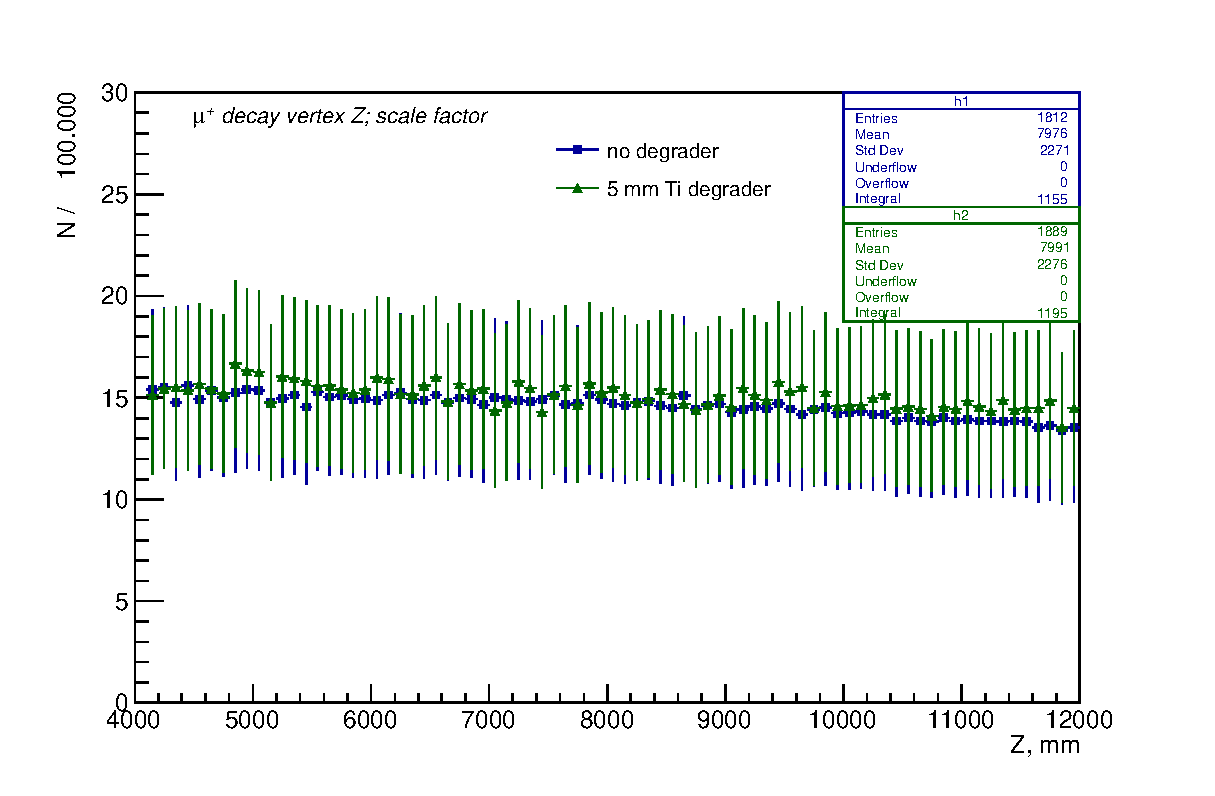
\includegraphics[width=0.8\textwidth]{pdf/figure_03701}
      }
    };
    % \node [text width=8cm, scale=1.0] at (14.5,0.5) {$\mu_B$, expected background mean};
    % \node [text width=8cm, scale=1.0, rotate={90}] at (1.5,7.5) { $S_{D}$, ``discovery'' signal strength  };
  \end{tikzpicture}
  \caption{
    \label{fig:pion_stop_time}
    The ratio of the Z vertex distributions - the scale factor
  }
\end{figure}

The scale factor coming out of the simulation is $SF = 15.0 \pm 1$ , consistent with the back-of-the-envelope
estimate of
$$
            SF = 1/(1 - exp^{-T_{max}/\tau}) = 15.15 ~~,
$$
where $T_{max} = 150$ ns and $\tau = 2197$ ns, the muon lifetime at rest. The [assigned] uncertainty also covers
the  range of the DF variations as a function of the decay vertex Z coordinate.
Therefore constraining the muon proper decay time in the detector to 150 ns improves the simulation efficiency
by a factor of 15 w/o introducing extra event-dependent weights.

Comparison between the momentum distributions of positrons produced using the "enhanced rate" simulation
of DIF to the default simulation is shown in Figure~\ref{figure:dif_pos_momentum}. The two distributions
are practically identical.

\begin{figure}[H]
  \begin{tikzpicture}
    \node[anchor=south west,inner sep=0] at (0,0.) {
      % \node[shift={(0 cm,0.cm)},inner sep=0,rotate={90}] at (0,0) {}
      \makebox[\textwidth][c] {
        \includegraphics[width=0.7\textwidth]{png/bmup5b0s24r0000_vs_bmup5b0s25r0000_positron_momentum}
      }
    };
    % \node [text width=8cm, scale=1.0] at (14.5,0.5) {$\mu_B$, expected background mean};
    % \node [text width=8cm, scale=1.0, rotate={90}] at (1.5,7.5) { $S_{D}$, ``discovery'' signal strength  };
  \end{tikzpicture}
  \caption{
    \label{figure:dif_pos_momentum}
    Positron momentum
  }
\end{figure}

Presented in Figure~\ref{figure:dif_muon_decay_time} comparison of the distributions of the $\mu^+$ decay
times shows however an interesting feature.

\begin{figure}[H]
  \begin{tikzpicture}
    \node[anchor=south west,inner sep=0] at (0,6.5) {
      % \node[shift={(0 cm,0.cm)},inner sep=0,rotate={90}] at (0,0) {}
      % \makebox[\textwidth][c] {
      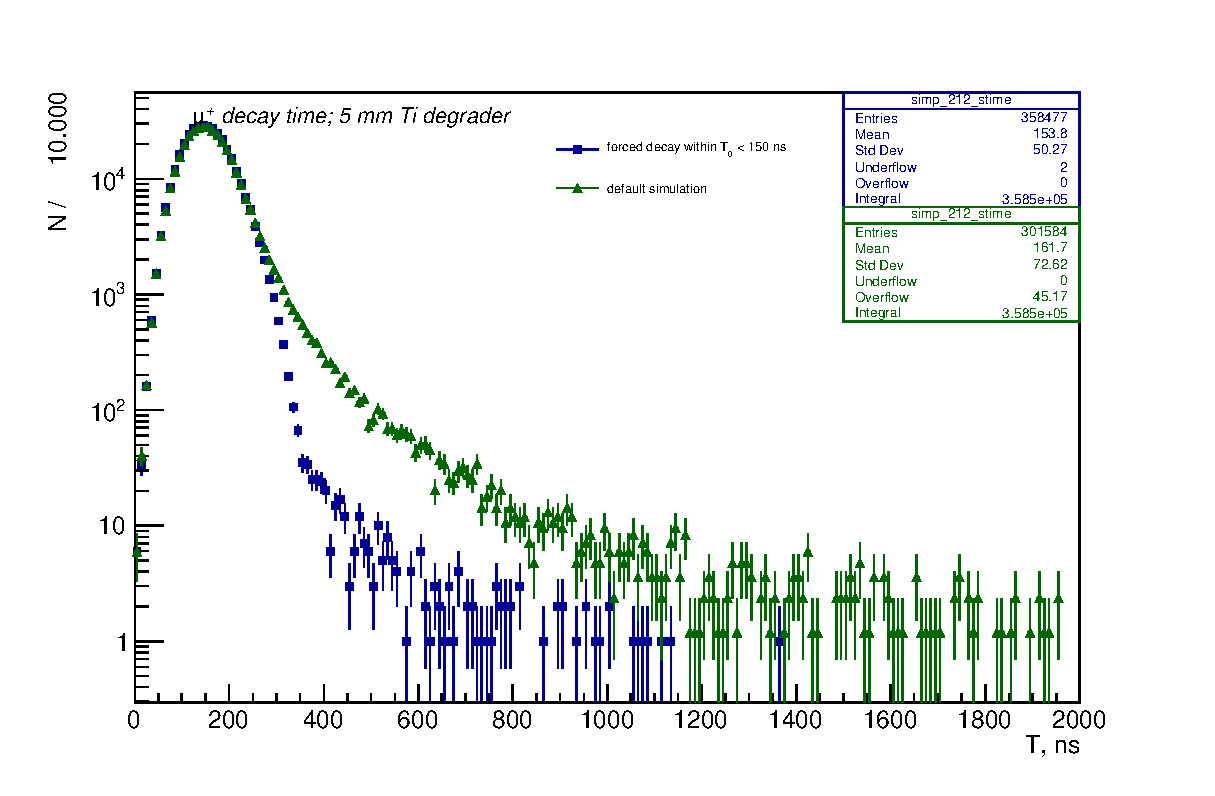
\includegraphics[width=0.54\textwidth]{pdf/figure_03412}
    };
    \node[anchor=south west,inner sep=0] at (10,6.5) {
      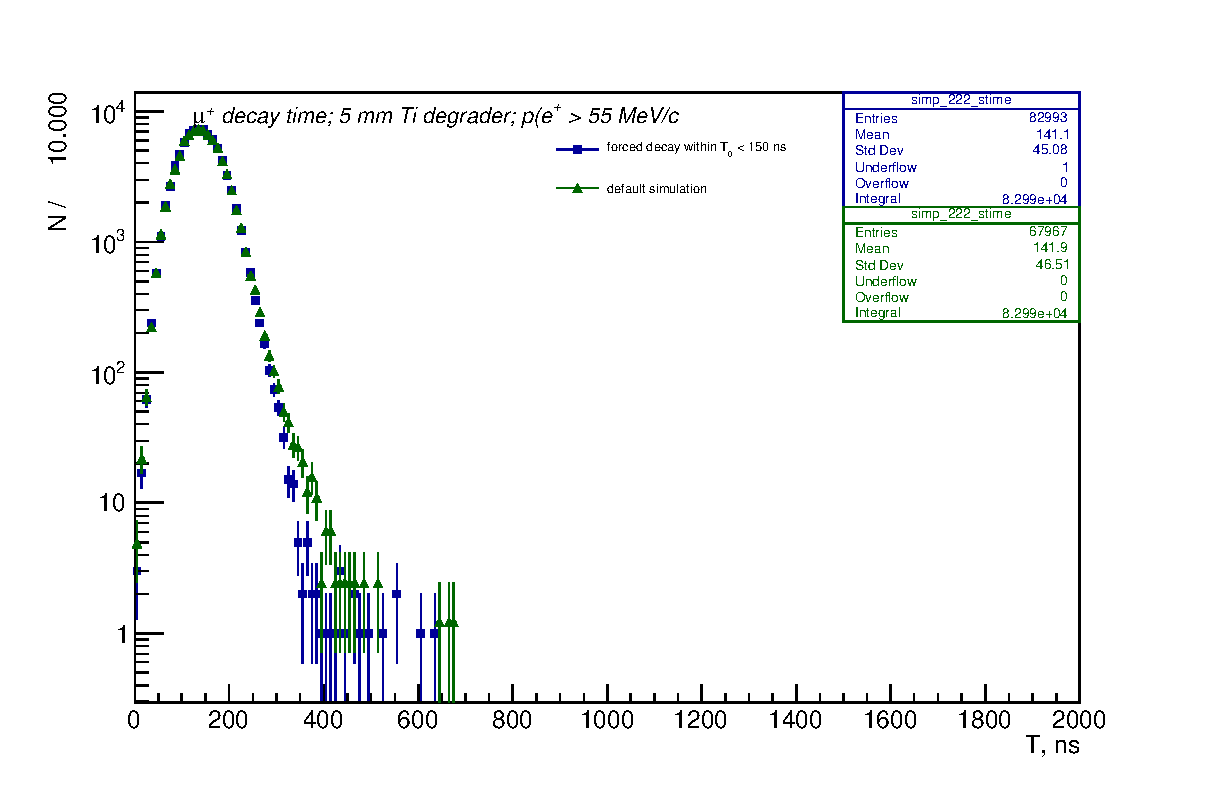
\includegraphics[width=0.54\textwidth]{pdf/figure_03422}
    };
    \node[anchor=south west,inner sep=0] at (0,0.) {
      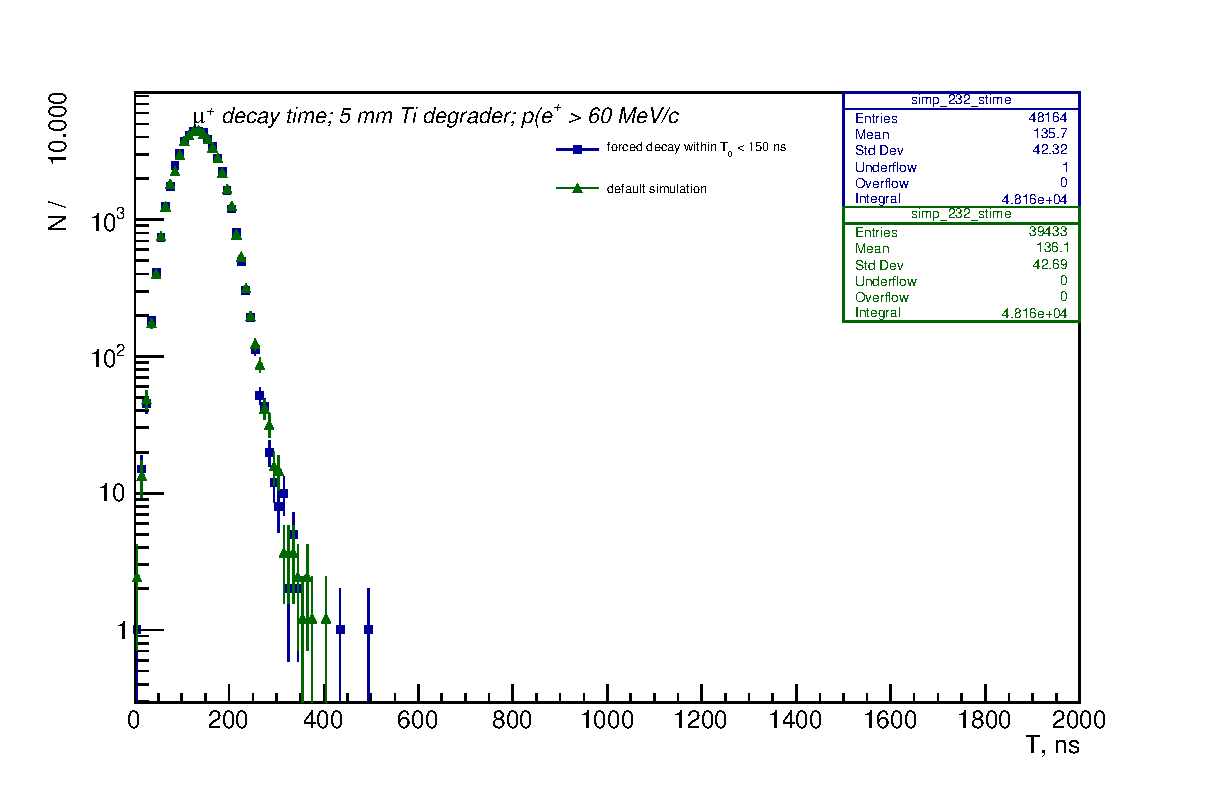
\includegraphics[width=0.54\textwidth]{pdf/figure_03432}
    };
    % \node [text width=8cm, scale=1.0] at (14.5,0.5) {$\mu_B$, expected background mean};
    % \node [text width=8cm, scale=1.0, rotate={90}] at (1.5,7.5) { $S_{D}$, ``discovery'' signal strength  };
  \end{tikzpicture}
  \caption{
    \label{figure:dif_muon_decay_time}
    Distributions of the $\mu^+$decay time in the DS for different momentum cuts: all momenta, p > 55 MeV/c,
    and p > 60 MeV/c. The distributions correspond to the default simulation and the simulation
    with the muon proper decay time truncated at $T_{max} = 150$ ns
  }
\end{figure}

The timing distribution for all positrons produced in muon decays in flight has a long tail.
Constraining the muon proper decay time at T0=150 ns has the tail reduced by an order of magnitude. 
For positrons with momenta above 55 MeV, the tail gets significantly reduced and it practically
disappears for events with positron p> 60 MeV/c.
The tail in the timing distribution has two components:

\begin{itemize}
\item
  muons reaching the DS with very low momenta, i.e. $P \simeq10 MeV/c$. Their arrival time to DS
  is large and even when decayed in the DS within 150 ns, still produce a timing tail.
  This category should be not be affected by the muon decay time truncation.
\item
  muons arriving to the DS fast enough, but losing their momentum in the degrader and traveling
  in the DS for more than 150 ns. Decays of these muons are not simulated when the muon decay time
  is truncated.
\end{itemize}

in both cases, as the muon mass is $M_{\mu}=105.5$ MeV, slow muons have very limited phase space
for producing positrons above $M_{\mu}/2$., and thus the impact of truncating the muon decay time
in the simulation for $p_{e^+} > M_{\mu}/2$ is very much suppressed .


%%% Local Variables:
%%% mode: latex
%%% TeX-master: "mu2e-xxxxx"
%%% End:
